\documentclass{beamer}

% Theme
\usetheme{Madrid}
\usecolortheme{default}

% Packages
\usepackage{amsmath,amssymb,amsfonts}
\usepackage{graphicx}
\usepackage{xcolor}
\usepackage{tikz}
\usepackage{mathtools}
\usepackage{tkz-euclide}
\usepackage{array}
\usepackage{multirow}
\usepackage{longtable}
\usepackage{lscape}
\usepackage{listings}
\lstset{
    basicstyle=\ttfamily\small,
    keywordstyle=\color{blue},
    commentstyle=\color{gray},
    stringstyle=\color{red},
    showstringspaces=false,
    breaklines=true
}

% Custom macros
\newcommand{\myvec}[1]{\begin{pmatrix}#1\end{pmatrix}}
\newcommand{\brak}[1]{\left( #1 \right)}
\newcommand{\augvec}[3]{%
  \left(\!\begin{array}{@{}*{#1}{r}|r@{}}#3\end{array}\!\right)
}



% Redefine \vec to bold letters only (no arrow)
\renewcommand{\vec}[1]{\mathbf{#1}}

\title{7.4.26}
\author{EE25BTECH11019 -- Darji Vivek M.}
\date{}

\begin{document}

\begin{frame}
\begin{titlepage}

\end{titlepage}
\end{frame}
\begin{frame}{Question}
\textbf{Question:}\\[2pt]
If two distinct chords, drawn from the point $(p,q)$ on the circle 
\[
x^2 + y^2 = px + qy
\]
(where $pq \ne 0$) are bisected by the $X$-axis, then which of the following is true?\\[2pt]
\begin{enumerate}
    \item $p^2 = q^2$
    \item $p^2 = 8q^2$
    \item $p^2 < 8q^2$
    \item $p^2 > 8q^2$
\end{enumerate}
\end{frame}

\begin{frame}{Solution}
Let
\begin{align}
\vec{P}=\myvec{p\\[2pt] q},\qquad 
\vec{c}=\frac{1}{2}\vec{P},\qquad 
r=\frac{1}{2}\sqrt{\vec{P}^\top\vec{P}}.
\end{align}
Hence, the circle in vector form is
\|\vec{x}-\vec{c}\|=r.\\
Let the midpoint of a chord through $\vec{P}$ lying on the $x$–axis be
\begin{align}
\vec{M}=\myvec{h\\[2pt]0},
\end{align}
and the other end of the chord be
\begin{align}
\vec{B}=2\vec{M}-\vec{P}.
\end{align}
Since $\vec{B}$ lies on the circle,
\begin{align}
\brak{\vec{B}-\vec{c}}^\top\brak{\vec{B}-\vec{c}}=r^2.
\end{align}
\end{frame}
\begin{frame}{Solution}
Substitute $\vec{B}=2\vec{M}-\vec{P}$ and $\vec{c}=\frac{1}{2}\vec{P}$:
\begin{align}
\brak{2\vec{M}-\frac{3}{2}\vec{P}}^\top\brak{2\vec{M}-\frac{3}{2}\vec{P}}
= \frac{1}{4}\vec{P}^\top\vec{P}.
\end{align}

Expand and simplify:
\begin{align}
4\vec{M}^\top\vec{M}-6\vec{M}^\top\vec{P}+\frac{9}{4}\vec{P}^\top\vec{P}
&= \frac{1}{4}\vec{P}^\top\vec{P} \\[2pt]
\implies 4\vec{M}^\top\vec{M}-6\vec{M}^\top\vec{P}+2\vec{P}^\top\vec{P} &= 0.
\end{align}

With $\vec{M}=\myvec{h\\[2pt]0}$,
\[
\vec{M}^\top\vec{M}=h^2,\qquad 
\vec{M}^\top\vec{P}=ph.
\]
Substitute:
\[
4h^2-6ph+2\vec{P}^\top\vec{P}=0.
\]
Divide by $2$:
\[
2h^2-3ph+\vec{P}^\top\vec{P}=0.
\]
\end{frame}
\begin{frame}{Solution}
For two distinct chords, this quadratic in $h$ must have two distinct real roots:
\begin{align}
\Delta &= 9p^2 - 8\vec{P}^\top\vec{P} > 0 \\[2pt]
&= 9p^2 - 8(p^2+q^2) > 0 \\[2pt]
\implies p^2 - 8q^2 > 0.
\end{align}

\[
\boxed{p^2 > 8q^2}
\]

Hence, option (d) is correct.
\end{frame}

\begin{frame}[fragile]{C Code: parallel\_funcs.c}
\begin{lstlisting}
https://github.com/vivekd03/ee1030-2025/blob/main/ee25btech11019/matgeo/7.4.26/codes/14.c
\end{lstlisting}
\end{frame}

\begin{frame}[fragile]{Python: Plotting Lines}
\begin{lstlisting}[language=Python, basicstyle=\ttfamily\scriptsize, keywordstyle=\color{blue}]
https://github.com/vivekd03/ee1030-2025/blob/main/ee25btech11019/matgeo/7.4.26/codes/14.py
\end{lstlisting}
\end{frame}

\begin{frame}{Pyhton plot}
\begin{figure}[h!]
    \centering
    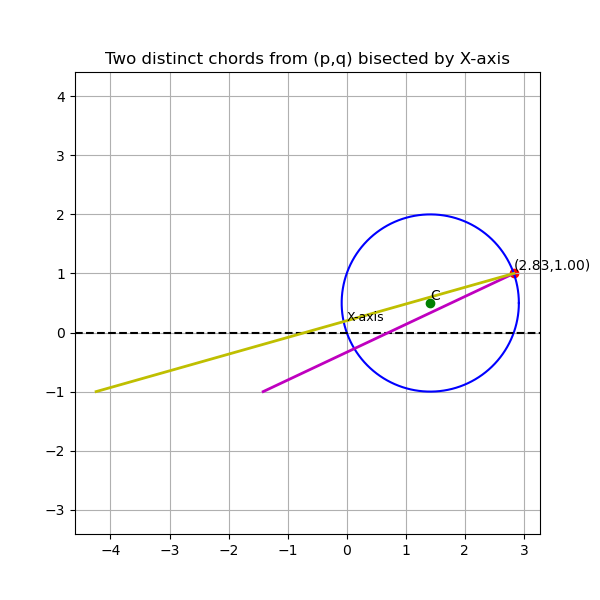
\includegraphics[width=0.75\textwidth]{figs/14.png}
    \caption{plot if p=2,q=2}
    \label{fig:example_image}
\end{figure}
\end{frame}

\end{document}